% =====================================================================
%  Compressed Sensing (D. L. Donoho, 2006)
%  Section-by-section explanation with small examples (study notes)
%  Overleaf: set main_en.tex as the Main document and compile with pdfLaTeX.
%  All numbers and figures come from code/cs_examples.py.
% =====================================================================
\documentclass[aspectratio=169,11pt]{beamer}
% --- Style: white background, plain blue titles, light blocks, page number bottom right ---
\usetheme{default}
\usepackage[utf8]{inputenc}
\usepackage[T1]{fontenc}
\usepackage{lmodern}
\usepackage{amsmath,amssymb,booktabs,graphicx,listings}
\graphicspath{{figures/}}
\setbeamertemplate{navigation symbols}{}
\setbeamertemplate{footline}[frame number]
\setbeamersize{text margin left=7mm,text margin right=7mm}
\setbeamerfont{frametitle}{size=\Large}

\definecolor{main}{HTML}{2A6EBB}      % blue: titles and definition blocks
\definecolor{warm}{HTML}{D9822B}      % orange: "note / SINDy" blocks
\definecolor{ok}{HTML}{1B8F6A}        % green: example blocks
\setbeamercolor{structure}{fg=main}
\setbeamercolor{frametitle}{fg=main}
% Blocks: light title, almost white body
\setbeamercolor{block title}{bg=main!10,fg=main!85!black}
\setbeamercolor{block body}{bg=main!3}
\setbeamercolor{block title example}{bg=ok!10,fg=ok!70!black}
\setbeamercolor{block body example}{bg=ok!3}
\setbeamercolor{block title alerted}{bg=warm!12,fg=warm!80!black}
\setbeamercolor{block body alerted}{bg=warm!4}

\lstset{language=Python,basicstyle=\ttfamily\footnotesize,keywordstyle=\color{main}\bfseries,
  commentstyle=\color{ok!70!black},stringstyle=\color{warm!80!black},showstringspaces=false,
  frame=single,rulecolor=\color{main!25},columns=fullflexible,keepspaces=true}

\newcommand{\en}[1]{\textit{#1}}          % technical term
\newcommand{\norm}[1]{\lVert #1\rVert}

\title[Compressed Sensing: study notes]{Compressed Sensing}
\subtitle{D.~L.~Donoho (2006) --- section by section, with small examples}
\author[L. Sadullaev]{Lazizbek Sadullaev \\ {\small (study notes)}}
\institute[WSU]{Department of Mathematics and Statistics, Washington State University}
\date{November 2026}

\AtBeginSection[]{
  \begin{frame}{Outline}
    \tableofcontents[currentsection]
  \end{frame}}

\begin{document}

\begin{frame}
  \titlepage
  \centering\footnotesize
  Source: D.~L.~Donoho, ``Compressed sensing'', \emph{IEEE Trans. Inf. Theory} 52(4), 1289--1306, 2006
\end{frame}


% ---------------------------------------------------------------------
\begin{frame}{What the paper is about --- in one sentence}
  \begin{block}{Main idea}
    If a signal is \en{sparse} (or \en{compressible}) in some basis, there is no need to measure all $m$ of its values:
    about $n\approx N\log m$ \textbf{random linear measurements} plus one \textbf{linear program} ($\ell_1$ minimization)
    suffice. Here $N$ is the number of important coefficients in the signal.
  \end{block}
  \begin{exampleblock}{Everyday example}
    A phone camera measures 12 million pixels, then JPEG throws most of them away (the signal compresses in a wavelet/DCT basis).
    \textbf{Question:} can we avoid measuring what will be thrown away anyway? The paper's answer: \textbf{yes}.
  \end{exampleblock}
  \begin{itemize}
    \item Previous paper (Basis Pursuit, 1998): $\ell_1$ as a \emph{principle}, no theory.
    \item This paper (2006): the \emph{theory} of when and why $\ell_1$ works.
  \end{itemize}
\end{frame}

\begin{frame}{Notation and the link to our project}
  \centering\small
  \begin{tabular}{@{}lll@{}}
    \toprule
    \textbf{In the paper} & \textbf{Meaning} & \textbf{In our SINDy project} \\
    \midrule
    $x\in\mathbb{R}^m$ & signal (e.g.\ an image) & --- \\
    $\Psi$, $\theta=\Psi^Tx$ & orthonormal basis, coefficients & library $\Theta$, coefficients $\Xi$ \\
    $\Phi$ ($n\times m$), $y=\Phi x$ & measurement matrix, $n$ measurements & --- (we do not choose it) \\
    $n<m$ & \en{underdetermined} & $m\gg p$, \en{overdetermined} \\
    $(P_1)$: $\min\norm{x}_1$, $\Phi x=y$ & Basis Pursuit & noiseless case of FBS-$\ell_1$ \\
    CS1--CS3 & matrix conditions & CS1 $\approx$ RLIP (Carlsson) \\
    \bottomrule
  \end{tabular}
  \medskip

  \raggedright
  \begin{alertblock}{Clash of letters --- careful!}
    In the paper $m$ = signal length, $n$ = number of measurements. In SINDy $m$ = number of time points (rows), $p$ = library columns.
    These slides use the paper's notation.
  \end{alertblock}
\end{frame}

% =====================================================================
\section{Introduction: transform sparsity and optimal recovery (\S I)}

\begin{frame}{\S I-A: Transform compression}
  \begin{block}{Model}
    $x\in\mathbb{R}^m$ is the signal, $\Psi$ an orthonormal basis (wavelet, Fourier, \dots). Coefficients:
    \[ \theta=\Psi^{T}x,\qquad x=\Psi\theta . \]
    The signal is \en{compressible} if a few coefficients of $\theta$ are large and the rest are very small.
  \end{block}
  \begin{exampleblock}{Example: Haar basis, $m=4$}
    $x=(3,\ 3,\ 1,\ 1)$ \ $\Longrightarrow$ \ $\theta=\Psi^Tx=(4,\ 2,\ 0,\ 0)$.
    \begin{itemize}
      \item In pixels (the Dirac basis): 4 nonzero numbers.
      \item In the Haar basis: only \textbf{2} --- the average and one ``difference''.
      \item Inverse: $\Psi\theta=(3,3,1,1)$, nothing is lost.
    \end{itemize}
  \end{exampleblock}
  {\small JPEG/JPEG-2000 work exactly like this: compute $\theta$, discard the small entries.}
\end{frame}

\begin{frame}{The $\ell_p$ ``norm'' and sparsity: why $p<1$?}
  \begin{block}{Definition}
    \[ \norm{\theta}_p=\Big(\sum_i|\theta_i|^p\Big)^{1/p},\qquad X_{p,m}(R)=\{\theta:\ \norm{\theta}_p\le R\}\ \ (\ell_p\ \text{ball}). \]
    For $0<p<1$ this is not a true norm (the triangle inequality fails), but it measures sparsity well.
  \end{block}
  \begin{exampleblock}{Example: two vectors, both with $\ell_2$ norm 1}
    \centering
    \begin{tabular}{@{}lccc@{}}
      \toprule
      & $p=2$ & $p=1$ & $p=0.5$ \\
      \midrule
      ``spike'' $(1,0,0,0)$ & 1 & 1 & 1 \\
      ``flat'' $(0.5,0.5,0.5,0.5)$ & 1 & 2 & \textbf{8} \\
      \bottomrule
    \end{tabular}
  \end{exampleblock}
  As $p$ decreases, a flat (dense) vector becomes ``expensive'' and a sparse one ``cheap''.
  So \textbf{$\norm{\theta}_p\le R$ with small $p$ = a strong sparsity} condition.
\end{frame}

\begin{frame}{N-term approximation: keeping the $N$ largest}
  \begin{block}{Fact (similar to (I.2) in the paper)}
    If $\theta\in X_{p,m}(R)$ and $\theta_N$ keeps the $N$ largest coefficients and zeros the rest, then
    \[ \norm{\theta-\theta_N}_2\ \le\ C_p\,R\,(N+1)^{1/2-1/p}. \]
  \end{block}
  \begin{exampleblock}{Example: $\theta_k=k^{-2}$ (i.e.\ $p=1/2$), $m=1000$}
    \centering
    \begin{tabular}{@{}rcc@{}}
      \toprule
      $N$ & error $\norm{\theta-\theta_N}_2$ & $N^{1/2-1/p}=N^{-3/2}$ \\
      \midrule
      10 & 0.01693 & 0.0316 \\
      20 & 0.00622 & 0.0112 \\
      40 & 0.00224 & 0.0040 \\
      \bottomrule
    \end{tabular}
  \end{exampleblock}
  Doubling $N$ cuts the error by $\approx2.72$; theory says $2^{3/2}=2.83$.
  \textbf{This is the ``ideal'' error}: achievable by someone who knows in advance which coefficients are large (an \en{oracle}).
\end{frame}

\begin{frame}{\S I-B: Optimal recovery --- setting up the problem}
  \begin{block}{Rules of the game}
    \begin{enumerate}
      \item \textbf{Information}: $n$ linear measurements $y=\Phi x$. $\Phi$ is chosen in advance, without seeing the signal (\en{nonadaptive}).
      \item \textbf{Algorithm} $A_n$: reconstructs $\hat x=A_n(y)$ from $y$.
      \item \textbf{Error}: the error on the worst signal.
    \end{enumerate}
    \[ E_n(X)=\inf_{\Phi,\,A_n}\ \sup_{x\in X}\ \norm{x-A_n(\Phi x)}_2 . \]
  \end{block}
  \begin{exampleblock}{Example: $m=2$, $n=1$}
    $\Phi=(1,\ 0)$: we measure only $x_1$. We know nothing about $x_2$ $\Rightarrow$ the worst error equals the largest possible value of $x_2$.
  \end{exampleblock}
  {\small Question: if $X$ is an ``$\ell_p$ ball'', how small can $E_n(X)$ be, and which $\Phi$ and which $A_n$ achieve it?}
\end{frame}

\begin{frame}{\S I-C: Four ``surprises''}
  \begin{enumerate}
    \item \textbf{Nonadaptive measurements are almost as powerful as an oracle.}
      Without knowing which coefficients are large, $n\approx N\log m$ measurements give the error of knowing the $N$ largest.
    \item \textbf{A good measurement is a ``hologram''.}
      The optimal $\Phi$ does not measure individual coefficients; every measurement mixes \emph{all} of them.
    \item \textbf{Adaptivity barely helps.}
      Choosing the next measurement based on previous ones improves the error only by a constant factor (Theorem 2).
    \item \textbf{For $p=1$ the results were known}, but indirectly (from approximation theory); practical $\Phi$ and algorithms were not.
  \end{enumerate}
  \begin{exampleblock}{Hologram example}
    ``Bad'' measurement: $y_1=\theta_1$ (one coefficient only). If the signal sits at $\theta_{57}$, we see nothing.
    ``Good'' measurement: $y_1=0.1\theta_1-0.3\theta_2+\dots+0.2\theta_m$ --- every sparse signal leaves some trace.
  \end{exampleblock}
\end{frame}

\begin{frame}{\S I-D: Geometry --- the Gel'fand width}
  \begin{block}{Definition}
    \[ d^n(X)=\inf_{L:\ \operatorname{codim}L=n}\ \sup\{\norm{x}_2:\ x\in X\cap L\}. \]
    $L$ is a subspace ``cut out by $n$ equations'' (i.e.\ the \en{null space} of some $\Phi$).
  \end{block}
  \textbf{Why does it matter?} $\Phi$ cannot see $x$ along its null space. If the null space cuts $X$ ``thinly'', the invisible part is small.
  \begin{block}{Theorem 3 (briefly)}
    For symmetric convex $X$: \quad $d^n(X)\ \le\ E_n(X)\ \le\ C\,d^n(X)$.
    \textbf{Best recovery error = ``thinness'' of the best null space} (up to a constant).
  \end{block}
  \begin{alertblock}{Intuition}
    Choosing $\Phi$ $=$ choosing a null space. A good null space contains \textbf{no sparse vectors}.
  \end{alertblock}
\end{frame}

\begin{frame}{Gel'fand width: the diamond example ($m=2$, $n=1$)}
  \begin{columns}[T]
    \begin{column}{0.42\textwidth}
      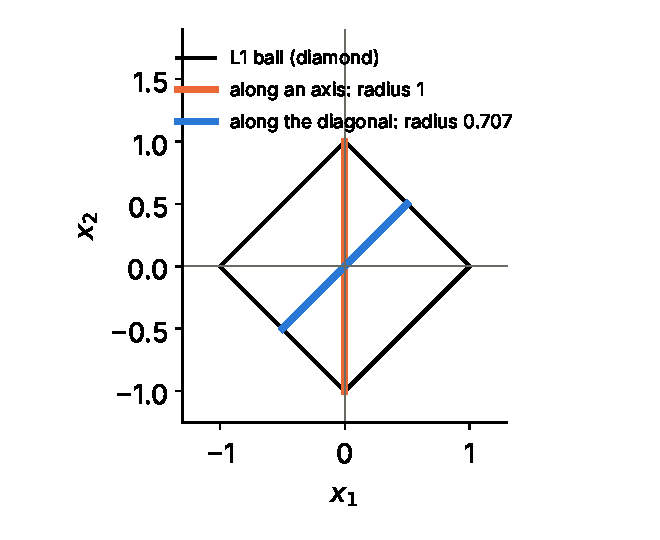
\includegraphics[width=\textwidth]{width_en.pdf}
    \end{column}
    \begin{column}{0.56\textwidth}
      \small
      $X$ = the $\ell_1$ ball (a diamond), one measurement $a^Tx$.
      \begin{exampleblock}{Two choices}
        \begin{itemize}
          \item $a=(1,0)$: null space = the $x_2$ axis. It meets the diamond at $(0,\pm1)$, \textbf{radius 1}.
          \item $a=(1,-1)$: null space = the diagonal. It meets it at $(\pm0.5,\pm0.5)$, \textbf{radius 0.707}.
        \end{itemize}
      \end{exampleblock}
      The second is better: its null space avoids the corners.
      In high dimension, for the $\ell_1$ ball (Kashin, Garnaev--Gluskin, Theorem 4)
      \[ d^n\asymp\min\Big(1,\ \sqrt{\log(m/n)/n}\Big). \]
      {\footnotesize E.g.\ $m=1000$, $n=100$: $0.152$; \ $n=400$: $0.048$.}
    \end{column}
  \end{columns}
\end{frame}

\begin{frame}{\S I-E, I-F: The ``mystery'' and the paper's results}
  \begin{block}{\S I-E: The mystery}
    Kashin--Garnaev--Gluskin proved that good null spaces \emph{exist} (random subspaces), but:
    \begin{itemize}
      \item there was no known way to check that a specific $\Phi$ is good;
      \item the optimal algorithm was not practical (combinatorial).
    \end{itemize}
  \end{block}
  \begin{block}{\S I-F: What the paper provides}
    \begin{enumerate}
      \item \textbf{Deterministic conditions} CS1--CS3: any $\Phi$ satisfying them is near-optimal (Theorem 7).
      \item \textbf{Almost all} random matrices satisfy CS1--CS3 (Theorems 6, 10).
      \item \textbf{A practical algorithm}: $\ell_1$ minimization (Basis Pursuit) is near-optimal (Theorems 8, 9).
    \end{enumerate}
  \end{block}
\end{frame}

\begin{frame}{The main result: Theorem 1}
  \begin{block}{Theorem 1 (simplified)}
    $0<p\le1$, $m\sim A\,n^\gamma$ ($\gamma>1$). Then
    \[ E_n\big(X_{p,m}(R)\big)\ \le\ C_p\,R\,\Big(\frac{n}{\log m}\Big)^{1/2-1/p}. \]
  \end{block}
  \begin{exampleblock}{Comparison with N-term approximation}
    \begin{itemize}
      \item Oracle (knowing the $N$ largest): error $\sim R\,N^{1/2-1/p}$.
      \item CS ($n$ random measurements): error $\sim R\,(n/\log m)^{1/2-1/p}$.
      \item They match $\iff$ $N\approx n/\log m$ $\iff$ \boxed{n\approx N\log m}.
    \end{itemize}
  \end{exampleblock}
  {\small Example: $m=10^6$, $N=1000$ important coefficients. $N\log m\approx13\,800$ measurements --- $1.4\%$ of $10^6$.}
\end{frame}

\begin{frame}{\S I-G: Potential applications (examples in the paper)}
  \small
  \begin{tabular}{@{}p{3.6cm}p{4.6cm}p{5.2cm}@{}}
    \toprule
    \textbf{Signal type} & \textbf{Basis} & \textbf{Measurements needed (relative to linear sampling)} \\
    \midrule
    Spectra (\en{bump algebra}) & wavelet & roughly the \textbf{cube root} \\
    Images (\en{bounded variation}) & wavelet & roughly the \textbf{square root} \\
    ``Cartoon'' images (smooth edges) & curvelet & roughly the \textbf{fourth root} \\
    \bottomrule
  \end{tabular}
  \normalsize
  \smallskip

  In numbers, $m=10^6$ pixels: \ $m^{1/2}=1000$, \quad $m^{1/3}=100$, \quad $m^{1/4}\approx32$.
  \begin{alertblock}{An honest remark}
    The formulas contain logarithmic factors. E.g.\ the abstract's $m^{1/4}\log^{5/2}m$: for $m=10^6$ it is $\approx22\,400$ (i.e.\ $\approx2\%$);
    for $m=10^4$ it is $\approx2\,600$ --- for small $m$ the log factor dominates. The results are \emph{asymptotic}.
  \end{alertblock}
\end{frame}

% =====================================================================
\section{Information: the CS conditions (\S II)}

\begin{frame}{\S II-A: Three conditions CS1--CS3 (simplified)}
  The columns of $\Phi$ are normalized; $J$ is a ``small'' index set, $|J|<\rho\,n/\log m$; $\Phi_J$ are those columns.
  \begin{block}{CS1: small groups are linearly independent}
    The smallest singular value of $\Phi_J$ is $\ge\eta_1>0$ (uniformly over all small $J$).
  \end{block}
  \begin{block}{CS2: combinations of small groups ``look like noise''}
    For $v\in\operatorname{range}(\Phi_J)$: \ $\norm{v}_1\ \ge\ \eta_2\sqrt n\,\norm{v}_2$.
  \end{block}
  \begin{block}{CS3: the remaining columns cannot rebuild $\Phi_J$ ``cheaply''}
    The smallest $\ell_1$ cost of writing a vector of $\operatorname{range}(\Phi_J)$ using columns outside $J$
    is not much smaller than $\norm{v}_1$ (bounded below with a factor $\eta_3/\sqrt{\log(m/n)}$).
  \end{block}
  {\footnotesize The exact constants and expressions are in the paper; here we give the idea.}
\end{frame}

\begin{frame}{CS1 by example: what does a singular value measure?}
  \begin{block}{Singular value}
    $\sigma_{\min}(\Phi_J)=\min_{\norm{c}_2=1}\norm{\Phi_Jc}_2$. If it is small, some combination of the columns is almost zero, i.e.\ they are nearly linearly dependent.
  \end{block}
  \begin{exampleblock}{Numerical example ($n=50$ rows)}
    \centering
    \begin{tabular}{@{}lc@{}}
      \toprule
      Columns & $\sigma_{\min}$ \\
      \midrule
      5 columns of a random matrix (worst of 2000 draws) & 0.574 \\
      5 columns of a random matrix (average) & 0.792 \\
      $\phi_1$ and $\phi_1+0.01\phi_2$ (two nearly identical columns) & \textbf{0.007} \\
      \bottomrule
    \end{tabular}
  \end{exampleblock}
  \begin{itemize}
    \item If CS1 fails: $\Phi_J c\approx0$, so the null space contains a \textbf{sparse vector} supported on $J$ $\Rightarrow$ recovery is impossible.
    \item This is very close to the RLIP of Carlsson et al.: ``any $K$ columns are linearly independent''.
  \end{itemize}
\end{frame}

\begin{frame}{CS2 by example: the ratio of $\ell_1$ to $\ell_2$}
  \begin{block}{Fact}
    For $v\in\mathbb{R}^n$: \ $\norm{v}_2\le\norm{v}_1\le\sqrt n\,\norm{v}_2$.
    The left bound holds for a single ``spike''; the right bound when all components are equal.
  \end{block}
  \begin{exampleblock}{Ratio $\norm{v}_1/(\sqrt n\,\norm{v}_2)$, $n=50$}
    \centering
    \begin{tabular}{@{}lc@{}}
      \toprule
      $v$ & ratio \\
      \midrule
      spike $e_1=(1,0,\dots,0)$ & 0.141 \ $(=1/\sqrt{50})$ \\
      $v=\Phi_Jc$, random $\Phi$ (2000 trials, worst) & 0.682 \\
      $v=\Phi_Jc$, random $\Phi$ (average) & 0.803 \\
      theoretical value for a Gaussian vector, $\sqrt{2/\pi}$ & 0.798 \\
      \bottomrule
    \end{tabular}
  \end{exampleblock}
  \textbf{Meaning:} any combination of a small group of columns is ``evenly spread'', never a spike.
  So the $\ell_1$ norm treats them as ``expensive'' --- and $\ell_1$ minimization does not drift in the wrong direction.
\end{frame}

\begin{frame}{\S II-B: CS matrices are near-optimal (Theorem 7)}
  \begin{block}{Theorem 7 (briefly)}
    If $\Phi$ satisfies CS1--CS3, $y=\Phi x$, $x\in X_{p,m}(R)$, then \emph{any} $\hat x$ that lies in $X$ and matches $y$ satisfies
    \[ \norm{x-\hat x}_2\ \le\ C\,R\,(n/\log m)^{1/2-1/p}. \]
  \end{block}
  \textbf{Logic (\S III-A, the ``feasible point'' method):}
  \begin{itemize}
    \item $x$ and $\hat x$ are both in $X$ and $\Phi x=\Phi\hat x$ $\Rightarrow$ $x-\hat x\in\operatorname{null}(\Phi)$.
    \item For symmetric convex $X$, $x-\hat x\in2X$.
    \item So $\norm{x-\hat x}_2\le2\cdot\sup\{\norm{h}_2:\ h\in X\cap\operatorname{null}\Phi\}$ --- \textbf{2 $\times$ width}.
  \end{itemize}
  \begin{exampleblock}{In the diamond example}
    With $a=(1,-1)$ the width is $0.707$. Any two points consistent with the data are at distance $\le1.414$.
  \end{exampleblock}
\end{frame}

% =====================================================================
\section{Algorithms: optimal recovery (\S III)}

\begin{frame}{\S III: Three theoretical results}
  \begin{block}{Theorem 3: width $=$ optimal error}
    $d^n(X)\le E_n(X)\le C\,d^n(X)$ (seen in \S I-D).
  \end{block}
  \begin{block}{Theorem 1: the rate}
    $E_n(X_{p,m})\asymp R\,(n/\log m)^{1/2-1/p}$. Proof: duality, \en{entropy numbers} and Theorem 7 combined.
  \end{block}
  \begin{block}{Theorem 2: adaptivity does not help}
    $E_n(X)\le C_p\,E_n^{\text{adapt}}(X)$: choosing measurements sequentially, based on earlier results, gains only a constant.
  \end{block}
  \begin{exampleblock}{Intuition for adaptivity: the ``20 questions'' game}
    In 20 questions, choosing each question based on the answers helps enormously. Not here: a good null space works for all sparse signals \emph{at once}.
  \end{exampleblock}
\end{frame}

% =====================================================================
\section{Basis Pursuit: a practical algorithm (\S IV)}

\begin{frame}{\S IV-A: $(P_1)$ --- a linear program}
  \begin{block}{Two problems}
    \[
      (P_0):\ \min\norm{x}_0\ \ \text{s.t. }\Phi x=y \qquad\qquad (P_1):\ \min\norm{x}_1\ \ \text{s.t. }\Phi x=y
    \]
    $\norm{x}_0$ is the number of nonzero components.
  \end{block}
  \begin{itemize}
    \item $(P_0)$ is the real goal, but \textbf{combinatorial}: all supports must be tried.
          {\small Example: $m=256$, 8 nonzeros: $\binom{256}{8}\approx4\times10^{14}$ candidates.}
    \item $(P_1)$ is a \textbf{linear program} (the $x=u-v$, $u,v\ge0$ trick from the previous paper). Solved quickly.
  \end{itemize}
  \begin{alertblock}{The paper's key question (\S IV-B)}
    When is the solution of $(P_1)$ the same as the solution of $(P_0)$?
  \end{alertblock}
\end{frame}

\begin{frame}{\S IV-B: Theorem 8 --- equivalence of $\ell_0$ and $\ell_1$}
  \begin{block}{Theorem 8 (simplified)}
    Let $\Phi$ satisfy CS1--CS3. There is $\rho^*>0$ (depending only on the CS constants) such that:
    if a solution of $(P_0)$ has \textbf{at most $\rho^*n/\log m$} nonzeros, it is also the \textbf{unique} solution of $(P_1)$.
  \end{block}
  \textbf{Meaning:} if the signal is sparse enough, an NP-hard problem is solved \emph{exactly} by a linear program.
  \begin{exampleblock}{Our experiment: $m=256$, $n=64$, 8 nonzeros, random $\Phi$}
    \begin{itemize}
      \item $(P_1)$ solution: error $\norm{\hat x-x}_2=7\times10^{-14}$ --- \textbf{exact recovery}, 8 nonzeros.
      \item Minimum-$\ell_2$ solution: error $3.81$, \textbf{256} nonzeros.
      \item Compare: $N\log m=8\log256\approx44<64$.
    \end{itemize}
  \end{exampleblock}
\end{frame}

\begin{frame}{The experiment in a picture: a length-256 signal from 64 measurements}
  \centering
  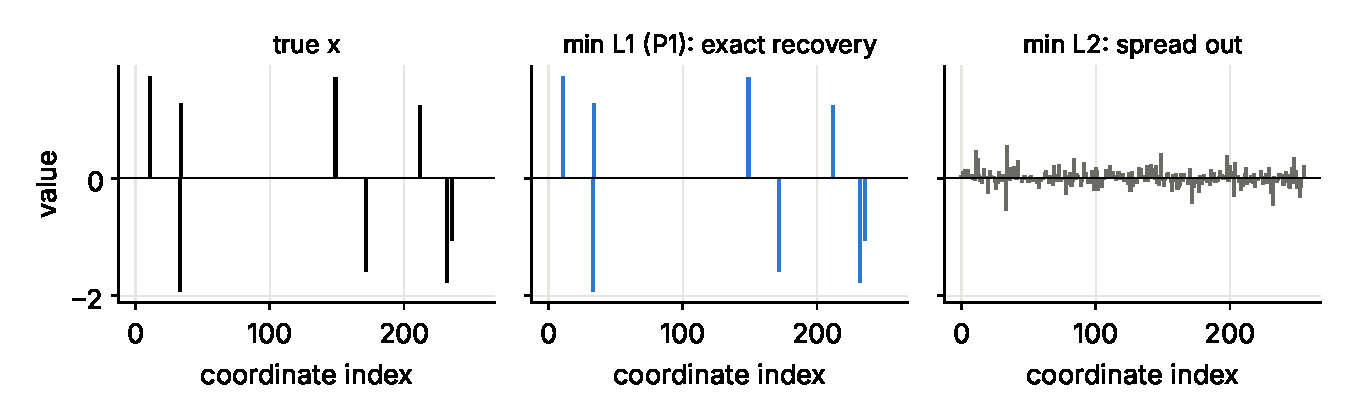
\includegraphics[width=0.85\textwidth]{cs_demo_en.pdf}

  \raggedright\small
  \begin{itemize}
    \item Left: the true signal (8 spikes). Middle: $(P_1)$ --- it coincides. Right: $\ell_2$ --- spread everywhere.
    \item $n=64<m=256$: four times fewer equations than unknowns, infinitely many solutions. Yet $\ell_1$ picked exactly the right one.
  \end{itemize}
\end{frame}

\begin{frame}{Small example: when $(P_1)$ succeeds and when it fails}
  $\Phi=\begin{pmatrix}1&0&0.707\\0&1&0.707\end{pmatrix}$ ($n=2$, $m=3$) --- the matrix from the previous paper.
  \begin{exampleblock}{Three signals}
    \centering
    \begin{tabular}{@{}lllc@{}}
      \toprule
      true $x$ & $y=\Phi x$ & $(P_1)$ result & correct? \\
      \midrule
      $(0,\ 0,\ 1.414)$ & $(1,\ 1)$ & $(0,\ 0,\ 1.414)$ & yes \\
      $(1,\ 0,\ 0)$ & $(1,\ 0)$ & $(1,\ 0,\ 0)$ & yes \\
      $(1,\ 1,\ 0)$ & $(1,\ 1)$ & $(0,\ 0,\ 1.414)$ & \textbf{no} \\
      \bottomrule
    \end{tabular}
  \end{exampleblock}
  \begin{itemize}
    \item 1 nonzero --- found. 2 nonzeros (with $n=2$) --- not found: the same $y$ can be written more cheaply with one atom.
    \item This is a ``tiny'' version of Theorem 8: the sparsity must be \emph{small enough} relative to $n$.
  \end{itemize}
\end{frame}

\begin{frame}{Why $(1,1,0)$ was not found: the dual certificate}
  \begin{block}{Optimality condition (from LP duality)}
    $x$ ($\operatorname{supp}=S$) solves $(P_1)$ $\iff$ there is a $w$ with
    \[ (\Phi^Tw)_i=\operatorname{sign}(x_i)\ \ (i\in S),\qquad |(\Phi^Tw)_i|\le1\ \ (i\notin S). \]
  \end{block}
  \begin{exampleblock}{In the example}
    \begin{itemize}
      \item $x=(0,0,1.414)$, $S=\{3\}$: $w=(0.707,\ 0.707)$ $\Rightarrow$ $\Phi^Tw=(0.707,\ 0.707,\ \mathbf{1})$. Condition holds \checkmark
      \item $x=(1,1,0)$, $S=\{1,2\}$: $(\Phi^Tw)_1=(\Phi^Tw)_2=1$ $\Rightarrow$ $w=(1,1)$ $\Rightarrow$ $\Phi^Tw=(1,\ 1,\ \mathbf{1.414})$. $1.414>1$ --- condition fails $\times$
    \end{itemize}
  \end{exampleblock}
  {\small\textbf{Proof idea in the paper (\S VII-C, D):} CS3 guarantees that such a $w$ (\en{sign-pattern embedding}) exists for every small support and sign pattern.}
\end{frame}

\begin{frame}{How many measurements? Success curves}
  \begin{columns}[T]
    \begin{column}{0.56\textwidth}
      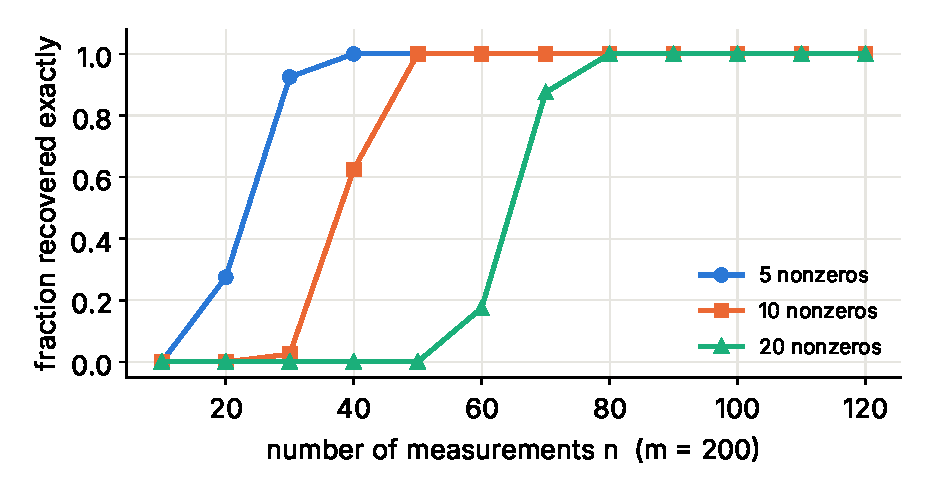
\includegraphics[width=\textwidth]{success_en.pdf}
    \end{column}
    \begin{column}{0.42\textwidth}
      \small
      $m=200$, 40 random trials per point. Fraction $=$ trials where $(P_1)$ recovered exactly.
      \medskip

      \centering
      \begin{tabular}{@{}ccc@{}}
        \toprule
        nonzeros & 100\% from & $N\log m$ \\
        \midrule
        5 & $n=40$ & 26 \\
        10 & $n=50$ & 53 \\
        20 & $n=80$ & 106 \\
        \bottomrule
      \end{tabular}
      \raggedright
      \medskip

      A sharp transition (\en{phase transition}): a small increase in $n$ takes the fraction from 0 to 1. $N\log m$ gives the right \emph{order}, not the exact constant.
    \end{column}
  \end{columns}
\end{frame}

\begin{frame}{\S IV-C: Theorem 9 --- compressible signals ($p<1$)}
  \begin{block}{Theorem 9 (simplified)}
    If $\Phi$ satisfies CS1--CS3 and $x\in X_{p,m}(R)$ (not exactly sparse, only compressible), the $(P_1)$ solution obeys
    \[ \norm{x-\hat x_1}_2\ \le\ C\,R\,(n/\log m)^{1/2-1/p}. \]
    Plain $\ell_1$ minimization achieves the \textbf{optimal rate}.
  \end{block}
  \vspace{-2mm}
  \begin{columns}[T]
    \begin{column}{0.5\textwidth}
      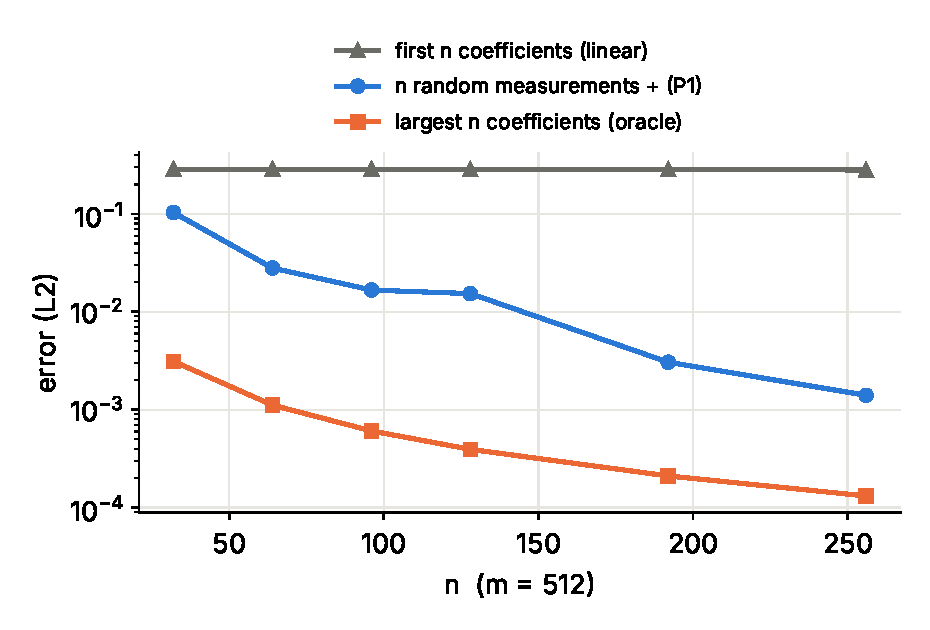
\includegraphics[width=0.88\textwidth]{compressible_en.pdf}
    \end{column}
    \begin{column}{0.48\textwidth}
      \small
      $|\theta|_{(k)}=k^{-2}$, $m=512$, random locations.
      \begin{itemize}
        \item \textbf{Gray}: measuring the first $n$ coordinates --- the error does not decrease ($\approx0.28$).
        \item \textbf{Blue}: CS + $(P_1)$ --- decreases fast.
        \item \textbf{Orange}: the oracle.
      \end{itemize}
      At $n=64$ the CS error $\approx$ the error of knowing the 8 largest; at $n=192$, about 33.
    \end{column}
  \end{columns}
\end{frame}

% =====================================================================
\section{Extensions and applications (\S V, \S VI)}

\begin{frame}{\S V-A: Tight frames}
  \begin{block}{Definition}
    $\Psi$ ($m\times M$, $M>m$) is a \en{tight frame} if $\Psi\Psi^T=I$. Then $x=\Psi(\Psi^Tx)$ and $\norm{\Psi^Tx}_2=\norm{x}_2$ (\en{Parseval}).
    Difference from an orthonormal basis: more columns, and they are not orthogonal.
  \end{block}
  \begin{exampleblock}{Example: the ``Mercedes'' frame, 3 vectors in $\mathbb{R}^2$ (120$^\circ$ apart)}
    $\Psi=\sqrt{2/3}\begin{pmatrix}0&-0.866&0.866\\1&-0.5&-0.5\end{pmatrix}$, \quad $\Psi\Psi^T=\begin{pmatrix}1&0\\0&1\end{pmatrix}$.
    \medskip

    $x=(1,2)$: \ $\theta=\Psi^Tx=(1.633,\ -1.524,\ -0.109)$, \ $\Psi\theta=(1,2)$, \ $\norm{\theta}^2=5=\norm{x}^2$.
  \end{exampleblock}
  {\small The paper: the proofs use only Parseval's identity, so all results carry over to tight frames (e.g.\ curvelets).}
\end{frame}

\begin{frame}{\S V-B: Weak $\ell_p$ balls}
  \begin{block}{Definition}
    Sort the coefficients by magnitude: $|\theta|_{(1)}\ge|\theta|_{(2)}\ge\dots$ \\
    $\theta\in w\ell_p(R)$ if $|\theta|_{(k)}\le R\,k^{-1/p}$ for all $k$.
  \end{block}
  \begin{exampleblock}{Example: $|\theta|_{(k)}=1/k$ (borderline $p=1$)}
    \begin{itemize}
      \item In weak $\ell_1$: $R=1$, since $1/k\le1\cdot k^{-1}$.
      \item Not in ordinary $\ell_1$ (for infinite $m$): $\sum_{k\le10}1/k=2.93$, $\sum_{k\le1000}1/k=7.49$, \dots\ $\to\infty$.
    \end{itemize}
  \end{exampleblock}
  {\small Weak $\ell_p$ is a slightly larger class; real signals (images) often fall into it. The results extend to it.}
\end{frame}

\begin{frame}{\S VI: Stylized applications}
  \begin{itemize}
    \item \textbf{\S VI-A, Bump algebra} (spectra: sums of smooth ``bumps'').
          The wavelet coefficients lie in an $\ell_1$-like ball. CS reaches the error of linear sampling with roughly the \textbf{cube root} as many measurements.
    \item \textbf{\S VI-B, Bounded variation images} (bounded total variation).
          Roughly the \textbf{square root}.
    \item \textbf{\S VI-C, Piecewise smooth images with edges} (``cartoon'' images, e.g.\ brain scans).
          With the curvelet tight frame, roughly the \textbf{fourth root}.
  \end{itemize}
  \begin{exampleblock}{Intuition: why a ``root''?}
    Linear sampling measures everywhere with the same density. But the information lives only in ``interesting'' places (bumps, edges).
    CS spends its measurements where the information is ``automatically'' --- even without knowing in advance where that is.
  \end{exampleblock}
\end{frame}

% =====================================================================
\section{Nearly all matrices are CS matrices (\S VII)}

\begin{frame}{\S VII: Random matrices (Theorems 6, 10)}
  \begin{block}{Construction}
    The columns of $\Phi$ are independent and uniformly distributed on the unit sphere $S^{n-1}$.
    In practice: take a matrix of Gaussian numbers and normalize each column.
  \end{block}
  \begin{block}{Theorem 10 (briefly)}
    For suitable $\eta_i,\rho>0$, when $n$ is large such a $\Phi$ satisfies CS1--CS3 with an \textbf{exponentially small} failure probability.
  \end{block}
  \textbf{Parts of the proof:}
  \begin{itemize}
    \item \S VII-A (CS1): the smallest singular value of $\Phi_J$ is not much below $\approx1-\sqrt{|J|/n}$.
          {\small Example: $|J|=5$, $n=50$: $1-\sqrt{0.1}=0.68$; in our experiment average $0.79$, worst $0.57$.}
    \item \S VII-B (CS2): \en{almost-spherical sections} (Kashin, Dvoretzky): on a random subspace $\ell_1$ and $\sqrt n\,\ell_2$ are nearly proportional.
    \item \S VII-C, D (CS3): \en{sign-pattern embedding} --- builds the dual certificate $w$ iteratively.
  \end{itemize}
\end{frame}

\begin{frame}{Why does randomness work?}
  \begin{block}{Intuition}
    A bad $\Phi$ is one whose null space contains a sparse vector. Sparse vectors are ``few'' (a thin set near the axes), while a random null space ``treats all directions equally''.
    The chance of hitting a sparse direction by accident is tiny.
  \end{block}
  \begin{exampleblock}{Analogy: the diamond example}
    In $\mathbb{R}^2$ a random line passes exactly through a corner of the diamond with probability 0. In high dimension there are many corners, but if the number of measurements is $n\gtrsim N\log m$, the risk disappears.
  \end{exampleblock}
  \begin{alertblock}{An important subtlety}
    Checking CS1--CS3 for a \emph{given} $\Phi$ is itself hard (combinatorial: all small $J$). The paper says ``random $\Rightarrow$ almost always good'', but gives no certificate for a specific matrix.
  \end{alertblock}
\end{frame}

% =====================================================================
\section{Conclusion (\S VIII)}

\begin{frame}{\S VIII-A: Stability under noise}
  The paper: the results are \textbf{stable under small noise} in the measurements --- small noise gives a small reconstruction error.
  \begin{exampleblock}{Our experiment ($m=256$, $n=64$, 8 nonzeros, $(P_1)$ applied directly)}
    \centering
    \begin{tabular}{@{}cc@{}}
      \toprule
      $\norm{\text{noise}}_2$ & $\norm{\hat x-x}_2$ \\
      \midrule
      0 & 0.0000 \\
      0.001 & 0.0014 \\
      0.01 & 0.0137 \\
      0.1 & 0.1366 \\
      \bottomrule
    \end{tabular}
  \end{exampleblock}
  The error is \textbf{linear} in the noise ($\approx1.4\times$). For larger noise, BPDN/LASSO is used instead of $(P_1)$
  (later work: Donoho--Elad--Temlyakov 2006; Cand\`es--Romberg--Tao 2006).
\end{frame}

\begin{frame}{\S VIII-B, C: Alternative conditions and partial Fourier}
  \begin{block}{\S VIII-B: Theorem 11}
    Instead of CS1--CS3, two simpler conditions also suffice:
    \begin{itemize}
      \item \textbf{A1}: a null-space vector cannot ``concentrate'' on a small set (a \en{concentration} bound);
      \item \textbf{A2}: the intersection of the null space with the $\ell_1$ ball is ``thin'' (a width bound).
    \end{itemize}
    {\footnotesize This idea later became the \en{null space property} (NSP).}
  \end{block}
  \begin{exampleblock}{A1 in the diamond example}
    $a=(1,0)$: null space $=(0,t)$ --- all mass on one coordinate $\Rightarrow$ bad. \ $a=(1,-1)$: $(t,t)$ --- evenly split $\Rightarrow$ good.
  \end{exampleblock}
  \begin{block}{\S VIII-C: The partial Fourier ensemble}
    Cand\`es--Romberg--Tao: random rows of the Fourier matrix also work (important for MRI).
  \end{block}
\end{frame}

% =====================================================================
\section{Connection with our SINDy project}

\begin{frame}{Underdetermined CS vs overdetermined SINDy}
  \centering\small
  \begin{tabular}{@{}p{3.4cm}p{5cm}p{5cm}@{}}
    \toprule
    & \textbf{Compressed sensing} & \textbf{SINDy} \\
    \midrule
    Shape & $n<m$ (few equations) & rows $\gg$ columns \\
    Who chooses the matrix & we do, at random & nature (the trajectory) \\
    Columns & nearly orthogonal & strongly correlated \\
    Main difficulty & choosing among infinitely many solutions & support under noise \\
    Role of $\ell_1$ & finding the sparsest solution & sparsity + (bias) \\
    \bottomrule
  \end{tabular}
  \medskip

  \raggedright
  \begin{block}{What carries over, what does not}
    \begin{itemize}
      \item \textbf{Carries over:} the idea of a deterministic condition --- ``small column groups are linearly independent'' (CS1 $\approx$ RLIP).
      \item \textbf{Does not:} ``random matrix $\Rightarrow$ the condition holds'' (Theorem 10). Our $\Theta$ is not random.
    \end{itemize}
  \end{block}
\end{frame}

\begin{frame}{CS1 on our Lorenz library (our own computation)}
  $\Theta$: 10 columns ($1,x,y,z,x^2,xy,xz,y^2,yz,z^2$), 10\,000 rows, columns normalized. We tried every $J$.
  \begin{exampleblock}{$\sigma_{\min}(\Theta_J)$ for the worst $J$}
    \centering
    \begin{tabular}{@{}cll@{}}
      \toprule
      $|J|$ & $\sigma_{\min}$ & worst $J$ \\
      \midrule
      2 & 0.181 & $\{xy,\ y^2\}$ \\
      3 & 0.053 & $\{1,\ z,\ z^2\}$ \\
      4 & 0.048 & $\{x,\ y,\ xz,\ yz\}$ \\
      10 & 0.024 & all columns \\
      \bottomrule
    \end{tabular}
  \end{exampleblock}
  \begin{itemize}
    \item Compare: in a random $50\times200$ matrix the worst $|J|=5$ value is $0.57$ --- about 12 times better than ours.
    \item Mutual coherence: $0.967$ ($xy$ and $y^2$), because $x\approx y$ on the Lorenz attractor.
    \item $\{1,z,z^2\}$: $z$ is always positive and lies in $\approx[5,45]$, so $1$, $z$, $z^2$ are nearly dependent.
  \end{itemize}
\end{frame}

\begin{frame}{What this result tells us}
  \begin{enumerate}
    \item In the overdetermined case ($10\,000\times10$) CS1 \textbf{holds} ($\sigma_{\min}=0.024>0$) --- but the constant is very small.
    \item Guarantees usually carry a factor $1/\sigma_{\min}$ or $1/\sigma_{\min}^2$ $\Rightarrow$ noise can be amplified by $\approx40$--$1700$.
    \item So for SINDy the question is not ``does the condition hold?'' but \textbf{``how bad is the constant, and can it be improved?''}
  \end{enumerate}
  \begin{alertblock}{An idea for the draft}
    State the condition in the Target Theorem through $\sigma_{\min}(\Theta_J)$ and report its actual value for Lorenz (0.024--0.18).
    This checks the claim ``RLIP is easier in the overdetermined case'' with numbers.
  \end{alertblock}
\end{frame}

\begin{frame}{Questions that follow from this paper (for Donoho)}
  \begin{enumerate}
    \item \textbf{Deterministic condition.} \\
      {\small\itshape ``Your CS1 condition asks small column subsets to be uniformly well conditioned. In SINDy the design is a deterministic
      library along one trajectory; for Lorenz the worst three-column subset has smallest singular value about 0.05. Is a condition of this type,
      with explicit constants, the right object for an overdetermined guarantee?''}
    \item \textbf{Instead of randomness.} \\
      {\small\itshape ``Your Theorem 10 relies on random measurements. When we cannot randomize the design, is there a way to recover the benefit,
      for example by randomly subsampling time points or using several trajectories?''}
    \item \textbf{Bias.} \\
      {\small\itshape ``$\ell_1$ gives exact recovery in the noiseless underdetermined case, but under noise it shrinks coefficients. Do you see non-convex
      penalties such as MCP as the natural next step in the overdetermined regime?''}
  \end{enumerate}
\end{frame}

\begin{frame}{Summary: five main ideas}
  \begin{enumerate}
    \item \textbf{Transform sparsity}: the signal lies in an $\ell_p$ ball ($p\le1$) in the basis $\Psi$ $\Rightarrow$ the $N$ largest coefficients suffice.
    \item \textbf{Optimal recovery} $=$ \textbf{Gel'fand width}: the best measurement is one whose null space contains no sparse vector.
    \item \textbf{The main rate}: $n\approx N\log m$ nonadaptive measurements give the error of an oracle's $N$ coefficients; adaptivity does not help.
    \item The deterministic conditions \textbf{CS1--CS3} suffice; \textbf{random} matrices satisfy them almost always.
    \item \textbf{Basis Pursuit} ($\ell_1$, a linear program) recovers a sparse enough signal \emph{exactly} and a compressible one at the \emph{optimal} rate.
  \end{enumerate}
  \medskip
  \begin{alertblock}{One sentence for our project}
    CS is a random, underdetermined world; SINDy is a deterministic, overdetermined, correlated one. A CS1-type condition carries over,
    but its constant is small for us, and the bias of $\ell_1$ remains a problem under noise.
  \end{alertblock}
\end{frame}

% =====================================================================
\appendix
\section*{Appendix: code}

\begin{frame}[fragile]{Appendix A: new functions used in the code (1)}
  {\small\textbf{\texttt{np.linalg.svd(A, compute\_uv=False)}} --- singular values only (largest to smallest). Used for CS1.}
\begin{lstlisting}
A = np.array([[3.0, 0.0],
              [0.0, 1.0],
              [0.0, 0.0]])
print(np.linalg.svd(A, compute_uv=False))
\end{lstlisting}
\begin{lstlisting}
[3. 1.]
\end{lstlisting}
\end{frame}

\begin{frame}[fragile]{Appendix A: normalizing columns}
  \textbf{\texttt{np.linalg.norm(M, axis=0)}} --- the norm of each \emph{column}. Normalizing the columns: \texttt{M / norms}.
  This is how $\Phi$ and $\Theta$ are normalized in the code (every column has length 1).
\begin{lstlisting}
M = np.array([[3.0, 0.0],
              [4.0, 2.0]])
print(np.linalg.norm(M, axis=0))
print(M / np.linalg.norm(M, axis=0))
\end{lstlisting}
\begin{lstlisting}
[5. 2.]
[[0.6 0. ]
 [0.8 1. ]]
\end{lstlisting}
  {\small The first column $(3,4)$ has length 5; normalized it is $(0.6,\ 0.8)$. NumPy divides each column by its own norm automatically (\en{broadcasting}).}
\end{frame}

\begin{frame}[fragile]{Appendix A: new functions used in the code (2)}
  \textbf{\texttt{rng.choice(m, k, replace=False)}} --- $k$ \emph{distinct} random numbers from $0,\dots,m-1$ (the support of a sparse signal).
\begin{lstlisting}
rng = np.random.default_rng(0)
print(rng.choice(8, 3, replace=False))
\end{lstlisting}
\begin{lstlisting}
[4 7 5]
\end{lstlisting}
  \textbf{\texttt{itertools.combinations(range(4), 2)}} --- all 2-element subsets (trying every $J$ in the Lorenz library).
\begin{lstlisting}
from itertools import combinations
print(list(combinations(range(4), 2)))
\end{lstlisting}
\begin{lstlisting}
[(0, 1), (0, 2), (0, 3), (1, 2), (1, 3), (2, 3)]
\end{lstlisting}
\end{frame}

\begin{frame}{Appendix B: files in the zip}
  \centering\small
  \begin{tabular}{@{}lp{8.2cm}@{}}
    \toprule
    File & What it is \\
    \midrule
    \texttt{main\_uz.tex}, \texttt{main\_en.tex} & the slides: Uzbek and English (Overleaf: pdfLaTeX) \\
    \texttt{main\_uz.pdf}, \texttt{main\_en.pdf} & compiled PDFs \\
    \texttt{figures/} & 4 figures, each in two languages (produced by the code) \\
    \texttt{code/cs\_examples.py} & all examples and figures \\
    \texttt{code/output.txt} & full output of the script (the numbers on the slides come from here) \\
    \bottomrule
  \end{tabular}
  \medskip

  \raggedright
  \textbf{Sections of the script:} A) $\ell_p$ norm; B) N-term approximation; C) Haar; D) Gel'fand width; E) the $2\times3$ example;
  F) main experiment; G) success curves; H) compressible signal; I) CS1, CS2; J) noise; K) Lorenz library; L) application numbers.
  \medskip

  \textbf{To run:} \texttt{cd code}, \ \texttt{python cs\_examples.py en}. Needs \texttt{numpy}, \texttt{scipy}, \texttt{matplotlib}. Time: $\approx25$ s.
\end{frame}

\end{document}
